where in the final step, all remaining tensors are contracted and combined into the final core $\Gt_4$. One can show that this procedure is \emph{exactly} equivalent to performing TT-SVD.

As expected, several other tensor networks are not covered in this chapter. In the next section, we briefly introduce some of them, which are notable generalizations of the Tucker and TT decompositions.
\subsection{Other decompositions: Tensor Ring, PEPS \& Hierarchical Tucker}

A first popular extension of Tensor Train is the Tensor Ring decomposition. 
\paragraph{Tensor Ring Decomposition}
The Tensor Ring (TR) decomposition is a generalization of the TT decomposition~\citep{zhao2016tensor}. Originally introduced in quantum physics, it has recently gained popularity in the machine learning community~\citep{wang2017efficient,wang2018wide,yuan2018higher}. While the TR decomposition is known to have some numerical stability issues~\citep{batselier2018trouble,chen2020tensor}, it generally requires fewer parameters and achieves better compression ratios than TT decomposition in practice~\citep{mickelin2020algorithms}. Let $\Xt\in\RR^{d_1\times\dots\times d_N}$
    be an $N$-th order tensor. Let 
    $\Gt_n\in\RR^{R_{n-1}\times d_n\times R_n}$ for $n\in[N]$ be the core tensors. 
    The rank-$R$ \emph{tensor ring decomposition} of the tensor $\Xt$ is given by
\begin{align*}
    \Xt_{i_1,\dots,i_N}=\hspace{0.25cm}\sum_{r_1=1}^{R_1}\dots\sum_{r_{N}=1}^{R_N}
    (\Gt_1)_{r_N,i_1,r_1} (\Gt_2)_{ r_1,i_2,r_2}\dots  (\Gt_{N-1})_{r_{N-2},i_{N-1},r_{N-1}} (\Gt_{N})_{r_{N-1},i_{N},r_N},
\end{align*}
for all indices $i_1\in[d_1],\cdots,i_N\in[d_N]$.
The TR decomposition can be represented in a tensor network notation for a fourth-order tensor as follows:
$$
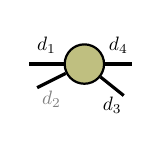
\begin{tikzpicture}[baseline=-0.5ex]
    \tikzset{tensor/.style = {minimum size = 0.5cm,shape = circle,thick,draw=black,inner sep = 0pt}, edge/.style = {thick,line width=.4mm},every loop/.style={}}
    \def\x{6}
    \def\y{0}
     \node[tensor,fill=green!50!red!50!white] (B) at (\x+1,\y) {$\Xt$};
    \draw[edge] (B) -- (\x+0.3,0) node [midway,above] {\scalebox{0.7}{\dimcolor{$d_1$}}};
    \draw[edge] (B) -- (\x+1.6,0) node [midway,above] {\scalebox{0.7}{\dimcolor{$d_4$}}};;
    \draw[edge] (B) -- (\x+0.4,-0.3) node [midway, below] {\scalebox{0.7}{\textcolor{gray}{$d_2$}}};;
    \draw[edge] (B) -- (\x+1.5,-0.4)node [midway, below] {\scalebox{0.7}{\dimcolor{$d_3$}}};;
\end{tikzpicture}=
\begin{tikzpicture}[baseline=\baseline]
    \tikzset{tensor/.style = {minimum size = 0.5cm,shape = circle,thick,draw=black,inner sep = 0pt}, edge/.style   = {thick,line width=.4mm},every loop/.style={}}
    \def\y{0}
    \def\x{0}
  \node[tensor,fill=red!30!white] (D) at (\x-1,\y){$\Gt_1$};
  \node[tensor,fill=red!50!white] (A) at (\x,\y){$\Gt_2$};
  \node[tensor,fill=blue!50!white] (B) at (\x+1,\y){$\Gt_3$};
   \node[tensor,fill=blue!20!white] (C) at (\x+2,\y){$\Gt_4$};
    \draw[edge](A) -- (\x,\y-0.7)node [midway,left] {\edgelabel{$d_2$}};
    \draw[edge](B) -- (\x+1,\y-0.7)node [midway,left] {\edgelabel{$d_3$}};
    \draw[edge](C) -- (\x+2,\y-0.7)node [midway,left] {\edgelabel{$d_4$}};
     \draw[edge](D) -- (\x-1,\y-0.7)node [midway,left] {\edgelabel{$d_1$}};
    \draw[edge](D) -- (A) node [midway,above] {\edgelabel{$R$}};
    \draw[edge](A) -- (B) node [midway,above] {\edgelabel{$R$}};
    \draw[edge](B) -- (C) node [midway,above] {\edgelabel{$R$}};
    \draw[edge] (D) to [out=145,in=35, distance=1cm] (C);
     \node[draw=none] () at (\x+0.5,\y+0.8) {\scalebox{0.7}{\dimcolor{$R$}}};
\end{tikzpicture}.
$$
As a special case of tensor ring decomposition, we can also obtain a rank-one decomposition by setting all the ranks equal to one:
$$
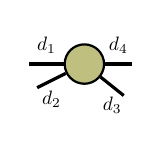
\begin{tikzpicture}[baseline=-0.5ex]
    \tikzset{tensor/.style = {minimum size = 0.5cm,shape = circle,thick,draw=black,inner sep = 0pt}, edge/.style = {thick,line width=.4mm},every loop/.style={}}
    \def\x{6}
    \def\y{0}
     \node[tensor,fill=green!50!red!50!white] (B) at (\x+1,\y) {$\Xt$};
    \draw[edge] (B) -- (\x+0.3,0) node [midway,above] {\scalebox{0.7}{\dimcolor{$d_1$}}};
    \draw[edge] (B) -- (\x+1.6,0) node [midway,above] {\scalebox{0.7}{\dimcolor{$d_4$}}};
    \draw[edge] (B) -- (\x+0.4,-0.3) node [midway, below] {\scalebox{0.7}{\dimcolor{$d_2$}}};
    \draw[edge] (B) -- (\x+1.5,-0.4)node [midway, below] {\scalebox{0.7}{\dimcolor{$d_3$}}};
\end{tikzpicture}=
\begin{tikzpicture}[baseline=\baseline]
    \tikzset{tensor/.style = {minimum size = 0.5cm,shape = circle,thick,draw=black,inner sep = 0pt}, edge/.style   = {thick,line width=.4mm},every loop/.style={}}
    \def\y{0}
    \def\x{0}
  \node[tensor,fill=red!30!white] (D) at (\x-1,\y){$\gb_1$};
  \node[tensor,fill=red!50!white] (A) at (\x,\y){$\gb_2$};
  \node[tensor,fill=blue!50!white] (B) at (\x+1,\y){$\gb_3$};
   \node[tensor,fill=blue!20!white] (C) at (\x+2,\y){$\gb_4$};
    \draw[edge](A) -- (\x,\y-0.7)node [midway,left] {\edgelabel{$d_2$}};
    \draw[edge](B) -- (\x+1,\y-0.7)node [midway,left] {\edgelabel{$d_3$}};
    \draw[edge](C) -- (\x+2,\y-0.7)node [midway,left] {\edgelabel{$d_4$}};
     \draw[edge](D) -- (\x-1,\y-0.7)node [midway,left] {\edgelabel{$d_1$}};
\end{tikzpicture}
=
\xb^1\outprod\xb^2\outprod\xb^3\outprod\xb^4.
$$
\paragraph{Projected Entangled Pair States (PEPS)}
The family of Projected Entangled Pair States~(PEPS) has emerged as one of the generalizations of the TT decomposition to higher-order lattice structures in quantum physics~\citep{verstraete2004renormalization,orus2014practical}.
PEPS are tensor networks structured as two-dimensional arrays of fifth-order core tensors. The following is the PEPS tensor diagram  corresponding to a $4\times 4$ square lattice:
$$
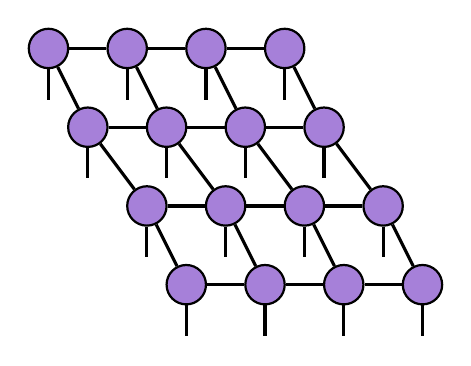
\begin{tikzpicture}[baseline=-0.5ex]
    \tikzset{tensor/.style = {minimum size = 0.5cm,shape = circle,thick,draw=black,inner sep = 0pt}, edge/.style = {thick,line width=.4mm},every loop/.style={}}
    \def\x{6}
    \def\y{0}
     \node[tensor,fill=red!30!blue!50!white] (A) at (\x,\y) {};
     \node[tensor,fill=red!30!blue!50!white] (B) at (\x+1,\y) {};
     \node[tensor,fill=red!30!blue!50!white] (C) at (\x+2,\y) {};
     \node[tensor,fill=red!30!blue!50!white] (D) at (\x+0.5,\y-1) {};
     \node[tensor,fill=red!30!blue!50!white] (E) at (\x+1.5,\y-1) {};
     \node[tensor,fill=red!30!blue!50!white] (F) at (\x+2.5,\y-1) {};
     \node[tensor,fill=red!30!blue!50!white] (G) at (\x+1.25,\y-2) {};
     \node[tensor,fill=red!30!blue!50!white] (H) at (\x+2.25,\y-2) {};
    \node[tensor,fill=red!30!blue!50!white] (I) at (\x+3.25,\y-2) {};
     \node[tensor,fill=red!30!blue!50!white] (J) at (\x+3,\y) {};
     \node[tensor,fill=red!30!blue!50!white] (K) at (\x+3.5,\y-1) {};
     \node[tensor,fill=red!30!blue!50!white] (L) at (\x+4.25,\y-2) {};
     \node[tensor,fill=red!30!blue!50!white] (M) at (\x+1.75,\y-3) {};

     \node[tensor,fill=red!30!blue!50!white] (N) at (\x+2.75,\y-3) {};
     \node[tensor,fill=red!30!blue!50!white] (O) at (\x+3.75,\y-3) {};
     \node[tensor,fill=red!30!blue!50!white] (P) at (\x+4.75,\y-3) {};
     
     \draw[edge](A) --(B);
    \draw[edge](A) --(\x,\y-0.65);
    \draw[edge](A) --(D);
    \draw[edge](B) --(C);
    \draw[edge](B) --(\x+1,\y-0.65);
    \draw[edge](B) --(E);
    \draw[edge](D) --(E);
    \draw[edge](C) --(F);
    \draw[edge](C) -- (\x+2,\y-0.65);
    \draw[edge](E) --(F);
    \draw[edge](F) -- (\x+2.5,\y-1.65);
    \draw[edge](D) --(G);
    \draw[edge](D) -- (\x+0.5,\y-1.65);
    \draw[edge](G) --(H);
    \draw[edge](E) --(H);
    \draw[edge](E) -- (\x+1.5,\y-1.65);
    \draw[edge](H) --(I);
    \draw[edge](F) --(I);
    \draw[edge](G) -- (\x+1.25,\y-2.65);
    \draw[edge](H) -- (\x+2.25,\y-2.65);
    \draw[edge](I) -- (\x+3.25,\y-2.65);
    \draw[edge](C)--(J);
     \draw[edge](K)--(F);
    \draw[edge](I)--(L);
    \draw[edge](J)--(K);
    \draw[edge](K)--(L);
    \draw[edge](J) -- (\x+3,\y-0.65);
    \draw[edge](K) -- (\x+3.5,\y-1.65);
    \draw[edge](L) -- (\x+4.25,\y-2.65);
    \draw[edge](M)--(N);
    \draw[edge](N)--(O);
    \draw[edge](O)--(P);
    \draw[edge](G)--(M);
    \draw[edge](H)--(N);
    \draw[edge](I)--(O);
    \draw[edge](L)--(P);
    \draw[edge](M)--(\x+1.75,\y-3.65);
    \draw[edge](N)--(\x+2.75,\y-3.65);
    \draw[edge](O)--(\x+3.75,\y-3.65);
    \draw[edge](P)--(\x+4.75,\y-3.65);
\end{tikzpicture}
$$
\paragraph{Tree Tensor Networks/~Hierarchical Tucker Decomposition}
Another tensor network of particular interest is the Tree Tensor Networks~(TTN) or Hierarchical Tucker~(HT) decomposition, originally introduced in~\citep{hackbusch2009new, grasedyck2010hierarchical}. A key advantage of this tensor network is its higher expressive power compared to simpler models like the TT decomposition. The tensor network diagram for the HT decomposition of a fourth-order tensor is shown below:
$$
\begin{tikzpicture}[baseline=\baseline]
    \tikzset{tensor/.style = {minimum size = 0.5cm,shape = circle,thick,draw=black,inner sep = 0pt}, edge/.style   = {thick,line width=.4mm},every loop/.style={}}
    \def\y{0}
    \def\x{0}
    \node[tensor,fill=blue!30!red!50!white] (A) at (\x+0.5,\y+1) {};
    \node[tensor,fill=blue!30!red!50!white] (B) at (\x,\y) {};
  \node[tensor,fill=blue!30!red!50!white] (C) at (\x+1,\y){};
   \node[tensor,fill=blue!30!red!50!white] (D) at (\x-1,\y-1){};
   \node[tensor,fill=blue!30!red!50!white] (E) at (\x,\y-1){};
   \node[tensor,fill=blue!30!red!50!white] (F) at (\x+1,\y-1){};
   \node[tensor,fill=blue!30!red!50!white] (G) at (\x+2,\y-1){};
   \draw[edge](A) -- (B);
   \draw[edge](A) -- (C);
   \draw[edge](B) -- (D);
   \draw[edge](B) -- (E);
    \draw[edge](C) -- (F);
   \draw[edge](C) -- (G);
    \draw[edge](D) -- (\x-1,\y-1.65);
   \draw[edge](E) -- (\x,\y-1.65);
    \draw[edge](F) -- (\x+1,\y-1.65);
   \draw[edge](G) -- (\x+2,\y-1.65);
\end{tikzpicture}
$$







